\scanpage{6}

\diagram{\[\begin{array}{cc}
E&\operatorname{Symm}_k(\overset{\deleted{\unsure{\vee}}}{E})^{\vee}\\
P^r&\Phi^k(P^r).
\end{array}\]}
\[
\unsure{\delta}_{r,k}\in\Phi^{(k-1)(r+1)}\bigl(\Phi^k(P^r)\bigr)
\]
(discriminant)

défini au signe près

\margin{$\underbrace{k-1\quad k-1\qquad k-1}_{r+1\ \text{fois}}$
\quad $(k-1)(r+1)$}

section de $\underline O_{\Phi^k(P^r)}((k-1)(r+1))$

Considérons une section \inserted{$\varphi$} de $\Phi^k(P^r)$ sur $S$, elle
définit donc un \deleted{\unsure{hom.} $\Phi^k(P^r)$ \unsure{section de}}
faisceau inversible $\check M$ sur $S$, image inverse
de $\underline O_{\Phi^k(P^r)}(1)$] et
\deleted{\unsure{si} l'image \unsure{la section}}
\inserted{$\delta_{r,k}$ a comme}
\deleted{$M$ \unsure{est engendré par la}}
l'image réciproque une section \inserted{$\delta$} de
$\check M^{(k-1)(r+1)}$.
\margin{quotient de $\operatorname{Symm}_k(E)^\vee$,
\unsure{i.e. dual d'un} sous-faisceau $M$ \unsure{qui est facteur}
\unsure{de} $\operatorname{Symm}_k(E)$}
\figure{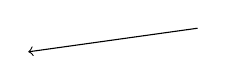
\begin{tikzpicture}\draw[->](2.4,.2)--(.25,-.1);\end{tikzpicture}}
Donc la section $\varphi$ \unsure{se remonte}
par $\Phi^k(P^r)_{\delta_{r,k}}$, i.e. $P^r_\varphi$ est \unsure{lisse} sur $S$,
sss $\delta$ est partout non nulle. Notons que
d'ailleurs, si $J=J_\varphi$ est l'idéal défini par $\varphi$
sur $P^r$, on a
\[
J\deleted{\unsure{_\varphi}}\simeq g^*(\overset{\deleted{\unsure{\vee}}}{M})(-k)
\]
\margin{\unsure{dualisons ici} $M\quad\check M$}
\figure{\begin{tikzpicture}\draw(0,0)..controls(.8,-1)and(.2,1.8)..(.65,1.2)
..controls(1,-.2)and(1.3,.2)..(1.45,1)
..controls(1.7,.3)and(2,.8)..(2.15,.9)
..controls(2.45,1.2)and(2.7,.7)..(2.9,.95);\end{tikzpicture}}
\[
\left[
\deleted{\underline O(-k)\otimes g^*(\unsure{E})\longrightarrow}
\underline O(-k)\otimes g^*(\operatorname{Symm}_k(E))\longrightarrow\underline O_{P^r}
\right.
\]
\margin{\unsure{par le choix d'un}}
d'où
\[
\underline O(\unsure{k|-k})\otimes g^*(M)\longrightarrow\underline O_{P^r}\quad-)
\]

\mspage{5}
